\chapter{Moderate convex wedges}
\label{ch:moderate}

In this chapter
we apply numerical boundary tracing to analyse corner rounding
in a moderate convex capillary wedge.
We include the borderline with the small-wedge regime
so that the full interval under consideration
is~$\pi/2 - \gamma \le \alpha < \pi/2$,
where $\alpha$~is the wedge half-angle
and $\gamma$~is the contact angle.
Specifically, we take a numerical solution
to the Laplace--Young equation~(\ref{eq:laplace-young}) in such a wedge
and seek rounded-corner curves along which
the contact condition~(\ref{eq:contact-boundary-condition})
remains satisfied.

At this point an objection will rightfully be raised:
Given that a numerical solver is needed
to generate the numerical wedge solution in the first place,
why bother with boundary tracing at all?
Indeed if boundary tracing can only produce
one rounding curve per numerical wedge solution,
why not directly apply the numerical solver to a rounded wedge?
This objection is addressed
in Section~\ref{sec:moderate.multiple},
where a novel observation is made
which enables multiple rounding curves to be produced by boundary tracing
per numerical wedge solution.

\thematicbreak

For simplicity we take the wedge to be of infinite extent.
The only physical parameter which appears
in the Laplace--Young equation~(\ref{eq:laplace-young})
and in the boundary condition~(\ref{eq:contact-boundary-condition})
is the capillary constant~$\capill$,
which has the dimensions of reciprocal area;
thus the sole length scale of the problem
is the capillary length
\begin{equation}
  L_0 = \frac{1}{\sqrt{\capill}}.
  \label{eq:capillary-length}
\end{equation}
We therefore put
\begin{align}
  T &= L_0 \scaled{T}, \label{eq:capillary-height-scaling} \\
  x &= L_0 \scaled{x}, \label{eq:capillary-x-scaling} \\
  y &= L_0 \scaled{y}, \label{eq:capillary-y-scaling}
\end{align}
noting that derivatives will transform according to
\begin{equation}
  \del = \scaleddel / L_0.
  \label{eq:capillary-del-scaling}
\end{equation}
Substituting and dropping \scalingmarks,
we obtain the dimensionless Laplace--Young equation
\begin{equation}
  \del \dotp \frac{\del T}{\sqrt{1 + (\del T)^2}} =  T
  \label{eq:scaled-laplace-young}
\end{equation}
within the scaled wedge,
whilst on the boundary we obtain the dimensionless contact condition
\begin{important}{equation}
  \normalvec \dotp \frac{\del T}{\sqrt{1 + (\del T)^2}} = \cos\gamma.
  \label{eq:scaled-contact-boundary-condition}
\end{important}

\section{Linearised corner rounding revisited}
\label{sec:moderate.linearised}

In this section we revisit the linearised corner rounding problem
for a right-angled wedge
considered by Anderson~\etal~%
  \cite{anderson-2007-boundary-tracing-ii-applications}.
We do so here to provide ourselves
with an explicit example of corner rounding (via boundary tracing)
in which the wedge solution is known analytically,
\emph{before} proceeding to the fully nonlinear case
where the known wedge solution will be a numerical one.

A similar revisit appeared in Section~2.1 of
the author's Honours thesis~\cite{li-2017-thesis-rounding-capillary-wedge};
there the analysis was conducted purely in polar coordinates,
rather than in the Cartesian coordinates and arc-length parametrisation
used here.

\subsection{Known solution}
\label{sec:moderate.linearised.known}

In the problem under consideration
the wedge is convex and right-angled, i.e.~$\alpha = \pi/4$.
The contact angle~$\gamma$ is assumed to be close to~$\pi/2$,
so that the capillary problem~(\ref{eq:scaled-laplace-young})
\&~(\ref{eq:scaled-contact-boundary-condition})
may be linearised by discarding~$(\del T)^2 \ll 1$.
The subsidiary height scaling
\begin{equation}
  T = U \cos\gamma
  \label{eq:helmholtz-height-scaling}
\end{equation}
removes the contact angle parameter,
leaving us with a linear BVP consisting of
the Helmholtz equation
\begin{equation}
  \del^2 U = U
  \label{eq:scaled-helmholtz}
\end{equation}
in the interior
together with the constant-flux condition
\begin{important}{equation}
  \normalvec \dotp \del U = 1
  \label{eq:scaled-contact-linearised}
\end{important}
on the boundary.

\begin{figure}
  \begin{minipage}[t]{0.4\textwidth}
    \centredfigurecontent[width=0.8\textwidth]{helmholtz-wedge-domain}{
      Right-angled wedge domain.
    }
  \end{minipage}
  \hfill
  \begin{minipage}[t]{0.55\textwidth}
    \centredfigurecontent{helmholtz-wedge-solution}{
      Known Helmholtz solution~(\ref{eq:scaled-helmholtz-solution})
      in a right-angled wedge.
    }
  \end{minipage}
\end{figure}

Whereas Anderson~\etal~\cite{anderson-2007-boundary-tracing-ii-applications}
used Cartesian coordinates aligned with the wedge walls,
here we align the positive $x$-axis so that it bisects the wedge
(for a logical extension to arbitrary wedge angles).
Thus the domain is the region~$\abs{y} < x$,
while the boundary consists of the wedge walls~$y = \pm x$ (with~$x \ge 0$),
as shown in Figure~\ref{fig:helmholtz-wedge-domain}.

As observed by Fowkes \&~Hood~\cite{fowkes-1998-surface-tension-effects-wedge},
the known solution to the Helmholtz BVP in this wedge is given by
\begin{important}{equation}
  U =
    \exp \roundbr*{\frac{-x+y}{\sqrt{2}}}
      +
    \exp \roundbr*{\frac{-x-y}{\sqrt{2}}},
  \label{eq:scaled-helmholtz-solution}
\end{important}
a superposition of capillary layers contributed by each wall
(Figure~\ref{fig:helmholtz-wedge-solution})

\subsection{Boundary tracing}
\label{sec:moderate.linearised.tracing}

Comparing the flux condition~(\ref{eq:scaled-contact-linearised})
to the generic~(\ref{eq:flux-boundary-condition})
(and noting that here we have $U$~in place of~$T$),
we see that the flux function is simply
\begin{equation}
  F = 1.
  \label{eq:helmholtz-flux-function}
\end{equation}
The derivatives of the known solution are
\begin{align}
  P &= \pder{U}{x} =
    \frac{1}{\sqrt{2}} \roundbr*{
      - \exp \roundbr*{\frac{-x+y}{\sqrt{2}}}
      - \exp \roundbr*{\frac{-x-y}{\sqrt{2}}}
    },
    \label{eq:helmholtz-gradient-x-component} \\[\tallspace]
  Q &= \pder{U}{y} =
    \frac{1}{\sqrt{2}} \roundbr*{
      + \exp \roundbr*{\frac{-x+y}{\sqrt{2}}}
      - \exp \roundbr*{\frac{-x-y}{\sqrt{2}}}
    },
    \label{eq:helmholtz-gradient-y-component}
\end{align}
and so the viability function is
\begin{align*}
  \Phi
  &= (\del U)^2 - F^2 \\
  &= \ee^{-\sqrt{2} (x - y)} + \ee^{-\sqrt{2} (x + y)} - 1.
    \yesnumber
    \label{eq:helmholtz-viability-function}
\end{align*}
Traced boundaries will only exist in the viable domain~$\Phi \ge 0$,
which may be written explicitly as
\begin{equation}
  x \le
    \frac{1}{\sqrt{2}}
    \log \roundbr*{2 \cosh \roundbr[\bulkysize]{\sqrt{2} \cdot y}}.
    \label{eq:helmholtz-viable-domain}
\end{equation}
Its border, the terminal curve~$\Phi = 0$,
is therefore given by
\begin{equation}
  x =
    \frac{1}{\sqrt{2}}
    \log \roundbr*{2 \cosh \roundbr[\bulkysize]{\sqrt{2} \cdot y}},
    \label{eq:helmholtz-terminal-curve}
\end{equation}
with the non-viable domain~$\Phi < 0$ lying strictly to its right
(Figure~\ref{fig:helmholtz-viable}).
Note how the terminal curve approaches the wedge walls~$y = \pm x$
as one moves away from the line of symmetry~$y = 0$.

\begin{figure}
  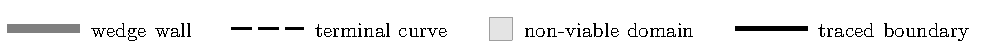
\includegraphics[width=\textwidth, trim=0 -10 0 0]{helmholtz-legend}
  \begin{minipage}[t]{0.5\textwidth}
    \centredfigurecontent[width=0.7\textwidth]{helmholtz-viable}{
      Non-viable domain~$\Phi < 0$.
    }
  \end{minipage}
  \begin{minipage}[t]{0.5\textwidth}
    \centredfigurecontent[width=0.7\textwidth]{helmholtz-traced-boundaries}{
      Traced boundaries obtained by integrating~%
        (\ref{eq:helmholtz-tracing-ode-arc-length-parametrisation-x})
      \&~%
        (\ref{eq:helmholtz-tracing-ode-arc-length-parametrisation-y}).
    }
  \end{minipage}
\end{figure}

The known solution~(\ref{eq:scaled-helmholtz-solution})
is insufficiently simple in form
for the boundary tracing ODE to be analytically solvable
under the coordinate parametrisations~$y = y (x)$ and~$x = x (y)$.
We therefore use the system~(\ref{eq:tracing-ode-arc-length-parametrisation-u})
\&~(\ref{eq:tracing-ode-arc-length-parametrisation-v})
for arc-length parametrisation,
which in the present case reduces to
\begin{important}{align}
  \tder{x}{s} &= \frac{-Q \pm P \sqrt{\Phi}}{(\del U)^2},
    \label{eq:helmholtz-tracing-ode-arc-length-parametrisation-x}
    \\[\tallspace]
  \tder{y}{s} &= \frac{+P \pm Q \sqrt{\Phi}}{(\del U)^2}.
    \label{eq:helmholtz-tracing-ode-arc-length-parametrisation-y}
\end{important}
Figure~\ref{fig:helmholtz-traced-boundaries}
shows the two branches of traced boundaries obtained
by integrating forward from various points
within the viable domain~(\ref{eq:helmholtz-viable-domain}).
The upper and lower branches have positive and negative slopes respectively.
As expected,
boundary tracing recovers the original boundaries of the Helmholtz BVP\@;
indeed the upper wedge wall~$y = +x$ is a traced boundary of the upper branch,
while the lower wedge wall~$y = -x$ is one of the lower branch.

\begin{figure}
  \centredfigurecontent{%
    helmholtz-traced-boundaries-patched%
  }{
    Domain boundaries~\figurestyle{thick black}
    patched together using traced boundaries~\figurestyle{grey}.
  }
\end{figure}

More interesting of course are the new boundaries obtained;
by construction, these also are curves
along which the boundary condition~(\ref{eq:scaled-contact-linearised}) holds.
More complicated boundaries can be constructed
by patching these curves together in an almost arbitrary fashion
(Figure~\ref{fig:helmholtz-traced-boundaries-patched});
the only restriction is that the boundary normal
have consistent orientation.
Since the flux in~(\ref{eq:scaled-contact-linearised}) is positive,
$U$~must be greater on the exterior,
and given the strictly negative $x$-derivative~%
  (\ref{eq:helmholtz-gradient-x-component}),
we may ensure consistent boundary orientation
by always identifying the region to the left as exterior.
Thus, each patching together of boundaries
will mark out a new domain to the right,
which also admits the solution~(\ref{eq:scaled-helmholtz-solution})
to the Helmholtz BVP~(\ref{eq:scaled-helmholtz})
\&~(\ref{eq:scaled-contact-linearised}).

\subsection{Corner rounding}
\label{sec:moderate.linearised.rounding}

While the domains produced in
Figure~\ref{fig:helmholtz-traced-boundaries-patched}
are most interesting,
their boundaries contain sharp corners,
incompatible with our goal of constructing a rounding of the wedge.
Recall that at any point \emph{strictly} within the viable domain,
two traced boundaries will cross at a non-zero angle,
forming a sharp corner if they are patched together.
To avoid corners we must therefore only perform patching
along the terminal curve, i.e.~at a terminal point.
Moreover, patching must only be performed at a critical terminal point,
for at an ordinary terminal point,
the two local traced boundaries form a cusp with inconsistent boundary normal
(see Section~\ref{sec:introduction.tracing}).
From Figure~\ref{fig:helmholtz-terminal-points}
we see that there is only one critical terminal point,
located at the intersection between
the terminal curve~(\ref{eq:helmholtz-terminal-curve})
and the line of symmetry~$y = 0$,
\begin{equation}
  (x_0, 0) = \roundbr*{\frac{\log 2}{\sqrt{2}}, \, 0}.
  \label{eq:helmholtz-critical-terminal-point}
\end{equation}
The local $U$-contour lies on the viable side of the terminal curve;
therefore the critical terminal point is of hyperbolic type,
and two smooth traced boundaries pass through it
(Figure~\ref{fig:helmholtz-traced-boundaries-hyperbolic-both}).
The portions to the left of the critical terminal point
eventually collide (at a non-zero angle) with the wedge walls,
so they do not form an acceptable rounding of the corner.
However, the portions to the right
can be shown to asymptotically approach the wedge walls;
patching them together gives the unique rounding curve for this problem
(Figure~\ref{fig:helmholtz-traced-boundaries-hyperbolic-rounding}).
We have therefore constructed a rounded-corner domain
which also admits the known solution~(\ref{eq:scaled-helmholtz-solution})
to the BVP~(\ref{eq:scaled-helmholtz})
\&~(\ref{eq:scaled-contact-linearised}).
To assess the effect that such a rounding will have
on the height rise,
we simply evaluate the known solution
along the walls of the original sharp-cornered wedge
and along the rounded corner;
the resulting height-rise profiles are shown in
Figure~\ref{fig:helmholtz-height-rise-profiles}.

\begin{figure}
  \centredfigurecontent[width=0.63\textwidth]{%
    helmholtz-terminal-points%
  }{
    $T$-contours which intersect the terminal curve~$\Phi = 0$.
  }
\end{figure}

\begin{figure}
  \newcommand*{\subfigurewidth}{0.45\textwidth}
  \newcommand*{\subfiguregraphicswidth}{0.55\textwidth}
  \centering
  \hspace*{\fill}
  \begin{subfigure}[t]{\subfigurewidth}
    \centredfigurecontent[width=\subfiguregraphicswidth]{%
      helmholtz-traced-boundaries-hyperbolic-both%
    }{%
      Two smooth boundaries
    }
  \end{subfigure}
    \hfill
  \begin{subfigure}[t]{\subfigurewidth}
    \centredfigurecontent[width=\subfiguregraphicswidth]{%
      helmholtz-traced-boundaries-hyperbolic-rounding%
    }{%
      Unique rounding of the corner
    }
  \end{subfigure}
  \hspace*{\fill}
  \caption{
    Traced boundaries through the critical terminal point~$(x_0, 0)$.
  }
  \label{fig:helmholtz-traced-boundaries-hyperbolic}
\end{figure}

\begin{figure}
  \centredfigurecontent[width=0.65\textwidth]{%
    helmholtz-height-rise-profiles%
  }{
    Height-rise profiles (parametrised by arc length)
    along the original wedge~\figurestyle{grey}
    and along the constructed rounding of the corner~\figurestyle{black}.
  }
\end{figure}

Of course the discovery of a single rounded corner
hardly completes an analysis of corner rounding.
Anderson~\etal~\cite{anderson-2007-boundary-tracing-ii-applications}
produced different roundings of the corner
by adding Bessel functions
to the known solution~(\ref{eq:scaled-helmholtz-solution})
before applying boundary tracing.
We note that such a superpositioning technique depends on
the linearity of the Helmholtz equation~(\ref{eq:scaled-helmholtz});
in the case of the Laplace--Young equation, which is nonlinear,
a different method is needed to produce multiple rounding curves.

\section{Nonlinear corner rounding}
\label{sec:moderate.nonlinear}

Having seen linearised corner rounding
for wedge half-angle~$\alpha = \pi/4$
and contact angle~$\gamma \approx \pi/2$,
we now consider the fully nonlinear Laplace--Young equation
over the moderate-wedge interval~$\pi/2 - \gamma \le \alpha < \pi/2$,
corresponding to convex capillary wedges whose corner height is bounded.
Since there are no exact solutions to work with,
the process consists of two parts:
first computing a numerical solution
to the BVP~(\ref{eq:scaled-laplace-young})
\&~(\ref{eq:scaled-contact-boundary-condition})
in a sharp-cornered wedge,
then applying boundary tracing to seek a rounded corner.

While corner rounding using a numerical wedge solution
was presented in Section~3.5
of the author's Honours thesis~\cite{li-2017-thesis-rounding-capillary-wedge}
(with some related theoretical discussion in Section~3.3),
we note a difference in objective with the work here.
In~\cite{li-2017-thesis-rounding-capillary-wedge},
the method was merely used
to assess the accuracy of asymptotic rounding curves
(obtained by applying boundary tracing to asymptotic solutions);
here, corner rounding of a numerical solution
is performed for its own sake.

\subsection{Numerical BVP solver}
\label{sec:moderate.nonlinear.numerical}

Numerical wedge solutions are computed
via finite elements in \software{Mathematica}.
The capillary BVP~(\ref{eq:scaled-laplace-young})
\&~(\ref{eq:scaled-contact-boundary-condition})
may be viewed as the steady-state diffusion problem
\begin{align}
  \del \dotp \squarebr[\bulkysize]{K (\del T) \del T} &= T,
    \label{eq:laplace-young-diffusion}
    \\[\tallspace]
  \normalvec \dotp \squarebr[\bulkysize]{K (\del T) \del T} &= \cos\gamma,
  \label{eq:contact-boundary-condition-diffusion}
\end{align}
with interior sink~$T$, boundary supply~$\cos\gamma$,
and nonlinear diffusion coefficient
\begin{equation}
  K (\del T) = \frac{1}{\sqrt{1 + (\del T)^2}}.
  \label{eq:laplace-young-diffusion-coefficient}
\end{equation}
\software{Mathematica~12}'s \code{NDSolve\`{}FEM\`{}} package
has built-in support for solving nonlinear BVPs.
When supplied with a nonlinear problem,
the built-in function \code{NDSolveValue}
iteratively solves a linearised version
according to Newton's method~%
  \cite{wolfram-2020-documentation-finite-element-programming}.%
\footnote{
  In~\cite{li-2017-thesis-rounding-capillary-wedge},
  an older version of \software{Mathematica} was used
  which could only solve linear BVPs.
  The nonlinearity was instead handled
  by a custom implementation of the slower fixed-point iteration,
  which linearises~(\ref{eq:laplace-young-diffusion})
  \&~(\ref{eq:contact-boundary-condition-diffusion})
  by using $K (\del T)$~evaluated from the previous step.
}
In the case of~(\ref{eq:laplace-young-diffusion})
\&~(\ref{eq:contact-boundary-condition-diffusion}),
we need simply set the \code{"DiffusionCoefficients"} property
to~$-K (\del T) \idenmat[2]$,
where $\idenmat[2]$~is the $2 \times 2$ identity matrix.
In all instances
we find that the default initial guess of the zero function
is sufficient for achieving convergence.

\subsubsection{Half-plane benchmarking}
\label{sec:moderate.nonlinear.numerical.half-plane}

Before computing wedge solutions,
we benchmark the numerical solver
against the known solution
for liquid against a single wall
(Figure~\ref{fig:half_plane-solution}).
In this problem,
the Laplace--Young equation~(\ref{eq:scaled-laplace-young})
is to be satisfied in the region~$x > 0$ occupied by the liquid,
while the contact condition~(\ref{eq:scaled-contact-boundary-condition})
is to be satisfied along the wall~$x = 0$.
The known solution,
called the \term{half-plane solution}~%
  \cite{anderson-2006-exact-solutions-laplace-young},
takes on the implicit form
\begin{equation}
  x (T) =
    \cosh^{-1} \roundbr*{\frac{2}{T}} - \sqrt{4 - T^2}
    - \cosh^{-1} \roundbr*{\frac{2}{h}} + \sqrt{4 - h^2},
  \label{eq:half-plane-solution}
\end{equation}
where
\begin{equation}
  \savecontent{
    h = \sqrt{2 (1 - \sin\gamma)}
  }{eq:half-plane-height}
\end{equation}
is the height rise at the wall~$x = 0$.

\begin{figure}
  \centredfigurecontent[width=0.48\textwidth]{%
    half_plane-solution%
  }{
    Known exact half-plane solution~(\ref{eq:half-plane-solution}).
  }
\end{figure}

Following Scott~\etal~\cite{scott-2005-computation-capillary-laplace-young},
we test our numerical solver in a $10 \times 1$~rectangle,
namely $0 < x < 10$, $-1/2 < y < 1/2$.
The contact condition~(\ref{eq:contact-boundary-condition-diffusion})
is applied along the wall-edge~$x = 0$,
while the natural Neumann condition
\begin{equation}
  \normalvec \dotp \squarebr[\bulkysize]{K (\del T) \del T} = 0
  \label{eq:natural-boundary-condition-diffusion}
\end{equation}
(corresponding to a non-wetting contact angle of~$\pi/2$)
is applied on the other three edges
so that the resulting numerical solution will both be $y$-independent
and vanish at infinity (approximated by~$x = 10$).

The rectangle is to be discretised into an unstructured triangular mesh,
and we use this opportunity to determine
a suitable level of mesh refinement to use
near the wall~$x = 0$, where the nonlinearity is significant.
Rather than specify an explicit refinement
(e.g.~a maximum cell area which increases with distance from the wall),
we use a minimalistic refinement strategy with only one rule:
the mesh vertices along~$x = 0$ must be spaced apart
by no more than~$\ell$, a chosen fine length scale.
Away from~$x = 0$ we simply let \software{Mathematica}'s
default meshing algorithm do its job,
resulting in a finite element mesh
that changes rapidly from fine to coarse
as one moves away from~$x = 0$
(Figure~\ref{fig:half_plane-mesh}).

\begin{figure}
  \centering
  \begin{subfigure}[t]{0.58\textwidth}
    \centredfigurecontent[trim=0 8 0 0]{half_plane-mesh-halves}{%
      Full mesh
    }
  \end{subfigure}
    \hfill
  \begin{subfigure}[t]{0.38\textwidth}
    \centredfigurecontent[trim=0 3 0 0]{half_plane-mesh-detail}{%
      Close-up of refinement
    }
  \end{subfigure}
  \caption{
    Half-plane finite element mesh with fine length scale~$\ell = 0.005$.
  }
  \label{fig:half_plane-mesh}
\end{figure}

\begin{table}
  \centering
  \begin{tabular}{
    S[table-format=1.3]
    S[table-format=4]
    S[table-format=1.4, round-mode=places, round-precision=4]
    S[table-format=+1.1e+1, round-mode=figures, scientific-notation=true]
  }
    \toprule
      {$\ell$}  &
      {\makecell{Mesh \\ elements}}  &
      {\makecell{Computed \\ height}}  &
      {\makecell{Relative \\ error}} \\
    \midrule
      0.001  &  6365  &  1.39754  &  -0.00304964 \\
      0.002  &  3459  &  1.39448  &  -0.00523459 \\
      0.005  &  1769  &  1.38838  &  -0.00958739 \\
      0.01   &  1190  &  1.38119  &  -0.0147169  \\
      0.02   &   899  &  1.36942  &  -0.023112   \\
      0.05   &   713  &  1.34613  &  -0.0397284  \\
      0.1    &   675  &  1.3332   &  -0.0489483  \\
      0.2    &   629  &  1.32062  &  -0.0579258  \\
    \bottomrule
  \end{tabular}
  \caption{
    Numerical results for half-plane wall height
    for~$\gamma = \SI{1}{\degree}$,
    for various refinement length scales~$\ell$.
  }
  \label{tab:half-plane-height-refinement-length}
\end{table}

Smaller contact angles are more computationally demanding
(as the slope near the wall is greater),
so we use~$\gamma = \SI{1}{\degree}$ for our benchmarking test.
For each chosen value of fine length scale~$\ell$,
a numerical solution is computed in the corresponding mesh,
with a computed wall height then obtained
by evaluating at~$(x, y) = (0, 0)$.
Table~\ref{tab:half-plane-height-refinement-length}
compares the computed heights
with the theoretical height~(\ref{eq:half-plane-height})
(which for~$\gamma = \SI{1}{\degree}$ evaluates to~$h = 1.4018$);
to obtain an error of less than~$\SI{1}{\percent}$
it suffices to use~$\ell = 0.005$.
For this choice of fine length scale,
our mesh consists of only 1769~elements.
This is a full order of magnitude lower than
Scott~\etal~\cite{scott-2005-computation-capillary-laplace-young}'s
mesh of 18000~elements, refined adaptively
with a mesh-element density proportional to the solution slope,
but which nevertheless only achieves an error of~$\SI{1.7}{\percent}$
in the computed wall height.
Clearly our minimalistic refinement strategy
offers a much more economical discretisation
by using a finer but much more localised refinement.
Figure~\ref{fig:half_plane-relative-error}
shows that the relative error
\begin{equation}
  \abs*{\frac{\textq{Computed~$T$}}{\textq{Exact~$T$}} - 1}
  \label{eq:half-plane-relative-error}
\end{equation}
for our numerical solution already decreases very rapidly
with increasing~$x$;
further small-scale refinement away from the wall~$x = 0$
is both unnecessary and wasteful.

\begin{figure}
  \centredfigurecontent[width=0.6\textwidth]{%
    half_plane-relative-error%
  }{
    Relative error along~$y = 0$
    for the numerical half-plane solution
    computed in the mesh with~$\ell = 0.005$.
  }
\end{figure}

\subsubsection{Wedge solutions}
\label{sec:moderate.nonlinear.numerical.wedge}

We now proceed to compute numerical solutions
in a wedge with interior angle~$2 \alpha$.
To approximate an infinite wedge,
the domain is taken to be the sector
$0 < r < 10$, $-\alpha < \phi < \alpha$
in polar coordinates.
The contact condition~(\ref{eq:contact-boundary-condition-diffusion})
is only applied along the two wedge walls~$\phi = \pm \alpha$.
To approximate a vanishing height rise at infinity,
the non-wetting zero-flux condition~%
  (\ref{eq:natural-boundary-condition-diffusion})
is applied instead along the far arc~$r = 10$.

Again the domain is discretised into an unstructured triangular mesh.
Since the aim is to use the resulting numerical wedge solutions
for boundary tracing,
we need to be able to evaluate first derivatives accurately;
therefore we require all mesh elements to have no more area than
the equilateral triangle of side length~$0.2$.
The minimalistic refinement strategy
of Section~\ref{sec:moderate.nonlinear.numerical.half-plane}
is applied along the two wedge walls~$\phi = \pm \alpha$.%
\footnote{
  In~\cite{li-2017-thesis-rounding-capillary-wedge},
  the mesh refinement was a function of the distance~$r$ from the corner.
  In hindsight this was a very poor choice,
  as the nonlinearity is significant
  along the entire length of the wedge walls,
  not just near the corner.
}
Since these walls are of length~$10$
(much greater than the length~$1$
of the refined wall for the half-plane benchmarking test),
we choose a more frugal fine length scale~$\ell = 0.01$
to avoid an excessive number of mesh elements.
For an $\alpha = \SI{40}{\degree}$~wedge,
the resulting mesh contains around~17000 elements
(Figure~\ref{fig:wedge_acute-mesh}).

\begin{figure}
  \centering
  \begin{subfigure}[t]{0.67\textwidth}
    \centredfigurecontent{wedge_acute-mesh-full}{%
      Full mesh
    }
  \end{subfigure}
    \hfill
  \begin{subfigure}[t]{0.27\textwidth}
    \centredfigurecontent[trim=0 {-0.6\textwidth} 0 0]{%
      wedge_acute-mesh-detail%
    }{%
      Close-up of refinement
    }
  \end{subfigure}
  \caption{
    Finite element mesh for an $\alpha = \SI{40}{\degree}$~wedge.
  }
  \label{fig:wedge_acute-mesh}
\end{figure}

\begin{table}
  \centering
  \begin{tabular}{
    S[table-format=2, table-space-text-post=\si{\degree}]
    S
    S[table-format=1.4e1]
    S[table-format=1.4, round-mode=places, round-precision=4]
    S[table-format=1.4e1]
    S[table-format=+1.1e+1, round-mode=figures, scientific-notation=true]
  }
    \toprule
      {$\gamma$}  &
      {\makecell{Theoretical \\ height}}  &
      {\makecell{Computed \\ height}}  &
      {\makecell{Theoretical \\ slope}}  &
      {\makecell{Computed \\ slope}}  &
      {\makecell{Relative \\ error}} \\
    \midrule
      30 \si{\degree}  &
        {$\infty$}  &  4.2413e2 &
        {$\infty$}  &  1.0691e5 &  {N/A} \\
      35 \si{\degree}  &
        {$\infty$}  &  3.3581e2 &
        {$\infty$}  &  8.4822e4 &  {N/A} \\
      40 \si{\degree}  &
        {$\infty$}  &  2.3533e2 &
        {$\infty$}  &  5.9586e4 &  {N/A} \\
      45 \si{\degree}  &
        {$\infty$}  &  1.0604e2 &
        {$\infty$}  &  2.6716e4 &  {N/A} \\
      50 \si{\degree}  &
        {finite}    &  2.0328   &
        {$\infty$}  &  1.6344e1 &  {N/A} \\
      55 \si{\degree}  &
        {finite}    &  1.5288  &
        1.97684     &  1.9758   &  -0.000509473 \\
      60 \si{\degree}  &
        {finite}    &  1.2548   &
        1.23778     &  1.2376   &  -0.000145694 \\
      65 \si{\degree}  &
        {finite}    &  1.0199   &
        0.872594    &  0.8726   &  -0.0000453895 \\
      70 \si{\degree}  &
        {finite}    &  0.8030   &
        0.628435    &  0.6284   &  -0.0000225007 \\
      75 \si{\degree}  &
        {finite}    &  0.5959   &
        0.439886    &  0.4399   &  -0.000012508 \\
      80 \si{\degree}  &
        {finite}    &  0.3946   &
        0.280581    &  0.2806   &  -7.90934e-6 \\
      85 \si{\degree}  &
        {finite}    &  0.1966   &
        0.136854    &  0.1369   &  -6.38643e-6 \\
    \bottomrule
  \end{tabular}
  \caption{
    Numerical results for corner height and corner slope
    in an $\alpha = \SI{40}{\degree}$~wedge,
    for various contact angles~$\gamma$.
    The critical angle (borderline case) is~$\gamma = \SI{50}{\degree}$.
  }
  \label{tab:convex-wedge-height-slope}
\end{table}

Numerical solutions may now be computed in the generated meshes
for various choices of wedge half-angle~$\alpha$ and contact angle~$\gamma$.
We recall that the height in the corner should be unbounded
if and only if~$\alpha < \pi/2 - \gamma$ (the small wedge regime),
and that the slope should be unbounded
if and only if~$\alpha \le \pi/2 - \gamma$.
Evidently infinite heights and slopes cannot be computed numerically,
but nevertheless if we apply our numerical solver in such cases,
we find that the singularities do manifest themselves
in the form of large quantities.
Table~\ref{tab:convex-wedge-height-slope}
shows the computed corner height and corner slope
in an $\alpha = \SI{40}{\degree}$~wedge;
indeed large heights and slopes are observed
as the contact angle~$\gamma$
decreases past the critical angle~$\pi/2 - \alpha = \SI{50}{\degree}$.
In the cases where both corner height and corner slope are finite,
the computed value of slope is in good agreement with the theoretical value
(given by the coefficient of~$r \cos\phi$
in the asymptotic form~(\ref{eq:moderate-wedge-asymptotic-solution})),
and we can be confident that the numerical solution
accurately represents the true solution in an infinite wedge.

In the borderline case~$\alpha = \pi/2 - \gamma$,
where the corner height is finite but the slope is infinite,
reservations about the near-corner validity of the numerical solutions
are allayed by a comparison with the asymptotic result
\begin{equation}
  T \asy
    T_0 - 2 \sqrt{\frac{x}{T_0}} + \frac{y^2}{4} \sqrt{\frac{T_0}{x}}
  \label{eq:borderline-wedge-asymptotic-solution}
\end{equation}
obtained by King~\etal~\cite{king-1999-laplace-young-near-corner};
here the corner height~$T_0$ is undetermined by the local analysis,
but when the numerically computed corner height is used,
indeed a good match is observed
as in Figure~\ref{fig:wedge_acute-borderline-asymptotic-comparison}.

\begin{figure}
  \newcommand*{\subfigurewidth}{0.45\textwidth}
  \centering
  \hspace*{\fill}
  \begin{subfigure}[t]{\subfigurewidth}
    \centredfigurecontent{%
      wedge_acute-borderline-asymptotic-comparison-symmetry%
    }{%
      Along line of symmetry~$y = 0$
    }
  \end{subfigure}
    \hfill
  \begin{subfigure}[t]{\subfigurewidth}
    \centredfigurecontent{%
      wedge_acute-borderline-asymptotic-comparison-wall%
    }{%
      Along wedge wall~$y = x \tan\alpha$
    }
  \end{subfigure}
  \hspace*{\fill}
  \caption{
    Comparison between the numerical solution~\figurestyle{solid}
    and the asymptotic result~%
      (\ref{eq:borderline-wedge-asymptotic-solution})~\figurestyle{dashed},
    for the borderline wedge~%
      $(\alpha, \gamma) = (\SI{40}{\degree}, \SI{50}{\degree})$.
  }
  \label{fig:wedge_acute-borderline-asymptotic-comparison}
\end{figure}

\begin{figure}
  \newcommand*{\subfigurewidth}{0.45\textwidth}
  \centering
  \begin{subfigure}[t]{\subfigurewidth}
    \centredfigurecontent{%
      wedge_acute-solution-borderline%
    }{%
      $\gamma = \SI{50}{\degree}$ (borderline case)
    }
  \end{subfigure}
    \hfill
  \begin{subfigure}[t]{\subfigurewidth}
    \centredfigurecontent{%
      wedge_acute-solution-moderate%
    }{%
      $\gamma = \SI{55}{\degree}$ (moderate regime)
    }
  \end{subfigure}
  \caption{
    Selected numerical solutions in an $\alpha = \SI{40}{\degree}$~wedge.
  }
  \label{fig:wedge_acute-solution}
\end{figure}

Thus, for the remainder of this chapter,
we may confidently use the numerical solutions
over the full interval~$\pi/2 - \gamma \le \alpha < \pi/2$
of convex wedges with a bounded corner height;
selected numerical solutions are shown
in Figure~\ref{fig:wedge_acute-solution}.
The small wedge case~$0 < \alpha < \pi/2 - \gamma$
we defer to Chapter~\ref{ch:small};
in that case both the corner height and corner slope are unbounded,
and a separate numerical treatment is required.

\subsection{Boundary tracing}
\label{sec:moderate.nonlinear.tracing}

Having obtained numerical solutions in sharp-cornered wedges,
we now proceed to the boundary tracing part
of the nonlinear corner rounding problem.
New boundaries are sought
along which the constant-contact-angle condition~%
  (\ref{eq:scaled-contact-boundary-condition})
holds.
Rewriting this condition as
\begin{important}{equation}
  \normalvec \dotp \del T = \cos\gamma \sqrt{1 + (\del T)^2}
  \label{eq:moderate-flux-boundary-condition}
\end{important}
and comparing it to the generic boundary condition~%
  (\ref{eq:flux-boundary-condition}),
it follows that the flux function is given by
\begin{equation}
  F = \cos\gamma \sqrt{1 + (\del T)^2}.
  \label{eq:moderate-flux-function}
\end{equation}
The viability function is therefore
\begin{align*}
  \Phi
  &= (\del T)^2 - F^2 \\
  &= \sin^2\gamma \, (\del T)^2 - \cos^2\gamma,
    \yesnumber
    \label{eq:moderate-viability-function}
\end{align*}
and the viable domain~$\Phi \ge 0$ can be written simply as
\begin{equation}
  \norm{\del T} \ge \cot\gamma.
  \label{eq:moderate-viable-domain}
\end{equation}
As a physical statement,
this asserts that the sought-after traced boundaries
will only exist in the region
where the known solution~$T$ is sufficiently steep;
specifically, at least as steep as a surface
which meets a vertical wall with contact angle~$\gamma$.
The terminal curve~$\Phi = 0$, or
\begin{equation}
  \norm{\del T} = \cot\gamma,
  \label{eq:moderate-terminal-curve}
\end{equation}
is the curve along which the known solution has
precisely the requisite steepness.

While polar coordinates would be appropriate
for an analytical description of the wedge,
the numerical wedge solutions are Cartesian-based.
Staying in Cartesian coordinates,
the components of the gradient vector
are the first derivatives
\begin{align}
  P &= \pder{T}{x},
    \label{eq:moderate-gradient-x-component} \\[\tallspace]
  Q &= \pder{T}{y},
    \label{eq:moderate-gradient-y-component}
\end{align}
which may easily be evaluated from our finite element solutions.
Since the work hereafter is purely numerical,
we use the arc-length parametrisation%
\footnote{
  In~\cite{li-2017-thesis-rounding-capillary-wedge},
  boundary tracing was performed in the coordinate parametrisation~$x = x (y)$.
  While the traced boundaries for the current problem
  indeed turn out to be never horizontal,
  we follow best practice here
  by making use of the arc-length parametrisation
  newly derived in Section~\ref{sec:curvilinear.tracing.arc-length}.
}~%
  (\ref{eq:tracing-ode-arc-length-parametrisation-u})
\&~%
  (\ref{eq:tracing-ode-arc-length-parametrisation-v}),
which in Cartesian coordinates reduces to
\begin{important}{align}
  \tder{x}{s} &= \frac{-Q F \pm P \sqrt{\Phi}}{(\del T)^2},
    \label{eq:moderate-tracing-ode-arc-length-parametrisation-x} \\[\tallspace]
  \tder{y}{s} &= \frac{+P F \pm Q \sqrt{\Phi}}{(\del T)^2}.
    \label{eq:moderate-tracing-ode-arc-length-parametrisation-y}
\end{important}
By numerically integrating forward from starting points
within the viable domain~(\ref{eq:moderate-viable-domain}),
we obtain the traced boundaries shown
in Figure~\ref{fig:wedge_acute-traced-boundaries}.
Qualitatively the situation is identical
to the linearised Helmholtz case
(compare Figure~\ref{fig:helmholtz-traced-boundaries});
there are two branches of traced boundaries
forming a curvilinear grid which fills the viable domain,
and the original wedge walls~$y = \pm x \tan\alpha$
are themselves traced boundaries.
As before, we can construct arbitrarily complicated domains
by patching the curves together,
ensuring consistent boundary orientation
by identifying the left side of each curve as the exterior
(Figure~\ref{fig:wedge_acute-traced-boundaries-patched}).

\begin{figure}
  \newcommand*{\legendoffsetheight}{0.34\textwidth}
  \centering
  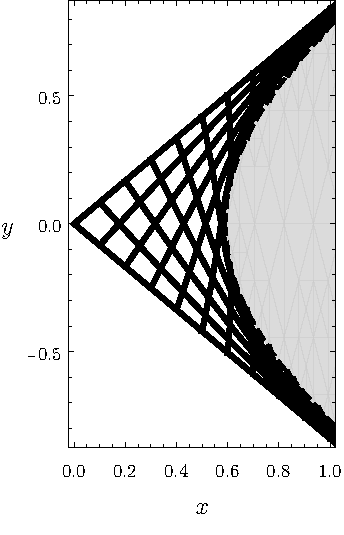
\includegraphics[width=0.4\textwidth]{wedge_acute-traced-boundaries}
  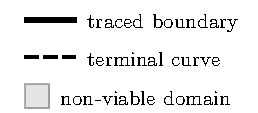
\includegraphics[
    width=0.3\textwidth,
    trim=0 {-\legendoffsetheight} 0 0,
  ]{wedge_acute-traced-boundaries-legend}
  \caption{
    Traced boundaries for~$\alpha = \SI{40}{\degree}$
    and~$\gamma = \SI{60}{\degree}$,
    obtained by integrating~%
      (\ref{eq:moderate-tracing-ode-arc-length-parametrisation-x})
    \&~%
      (\ref{eq:moderate-tracing-ode-arc-length-parametrisation-y}).
  }
  \label{fig:wedge_acute-traced-boundaries}
\end{figure}

\begin{figure}
  \centredfigurecontent{%
    wedge_acute-traced-boundaries-patched%
  }{
    Domain boundaries~\figurestyle{thick black}
    patched together using traced boundaries~\figurestyle{grey}.
    Similar to Figure~\ref{fig:helmholtz-traced-boundaries-patched},
    but not identical.
  }
\end{figure}

\begin{figure}
  \centredfigurecontent[width=0.65\textwidth]{%
    wedge_acute-terminal-points%
  }{
    $T$-contours which intersect the terminal curve~$\Phi = 0$.
    Similar to Figure~\ref{fig:helmholtz-terminal-points},
    but not identical.
  }
\end{figure}

A corner is formed by the two traced boundaries
that pass through any point \emph{strictly} within the viable domain,
so the search for a smooth curve which rounds off the wedge
again brings us to the terminal curve.
Inspecting how the $T$-contours cross the terminal curve
(Figure~\ref{fig:wedge_acute-terminal-points}),
we see that all the terminal points
for which~$y \ne 0$
are ordinary as before.
Only one critical terminal point~$(x, y) = (x_0, 0)$ exists,
located at the intersection
between the terminal curve~(\ref{eq:moderate-terminal-curve})
and the line of symmetry~$y = 0$.
Explicitly, $x = x_0$~is the unique solution to
\begin{equation}
  \eval*{-\pder{T}{x}}_{y=0} = \cot\gamma.
  \label{eq:moderate-critical-terminal-point}
\end{equation}
Again the local $T$-contour lies on the viable side of the terminal curve,
so the critical terminal point~$(x_0, 0)$ is of hyperbolic type.
Thus, as in the linearised Helmholtz case,
there are two smooth traced boundaries through~$(x_0, 0)$.
The portions to the left eventually meet the wedge at an angle,
but the portions to the right form a \term{candidate boundary}
which appears to round the corner
(Figure~\ref{fig:wedge_acute-traced-boundaries-hyperbolic-rounding}).

\begin{figure}
  \newcommand*{\subfigurewidth}{0.45\textwidth}
  \newcommand*{\subfiguregraphicswidth}{0.7\textwidth}
  \centering
  \hspace*{\fill}
  \begin{subfigure}[t]{\subfigurewidth}
    \centredfigurecontent[width=\subfiguregraphicswidth]{%
      wedge_acute-traced-boundaries-hyperbolic-both%
    }{%
      Two smooth boundaries
    }
  \end{subfigure}
    \hfill
  \begin{subfigure}[t]{\subfigurewidth}
    \centredfigurecontent[width=\subfiguregraphicswidth]{%
      wedge_acute-traced-boundaries-hyperbolic-rounding%
    }{%
      Candidate boundary
    }
  \end{subfigure}
  \hspace*{\fill}
  \caption{
    Traced boundaries through the critical terminal point~$(x_0, 0)$.
    Similar to Figure~\ref{fig:helmholtz-traced-boundaries-hyperbolic},
    but not identical.
  }
  \label{fig:wedge_acute-traced-boundaries-hyperbolic}
\end{figure}

\subsection{Rounding rate of approach}
\label{sec:moderate.nonlinear.approach}

In~\cite{li-2017-thesis-rounding-capillary-wedge},
it was shown (using a perturbation argument in polar coordinates)
that this candidate boundary
indeed approaches the original wedge walls asymptotically,
making it the unique rounding of the corner.
Here we extend this result by computing a rough estimate
for the rate of approach.

\begin{figure}
  \newcommand*{\subfigurewidth}{0.45\textwidth}
  \newcommand*{\subfiguregraphicswidth}{0.7\textwidth}
  \centering
  \hspace*{\fill}
  \begin{subfigure}[t]{\subfigurewidth}
    \centredfigurecontent[width=\subfiguregraphicswidth]{%
      wedge_acute-traced-boundaries-upper-branch%
    }{%
      Upper branch
    }
  \end{subfigure}
    \hfill
  \begin{subfigure}[t]{\subfigurewidth}
    \centredfigurecontent[width=\subfiguregraphicswidth]{%
      wedge_acute-traced-boundaries-lower-branch%
    }{%
      Lower branch
    }
  \end{subfigure}
  \hspace*{\fill}
  \caption{
    Traced boundaries segregated by branch.
  }
  \label{fig:wedge_acute-traced-boundaries-branches}
\end{figure}

\begin{figure}
  \centredfigurecontent[width=0.3\textwidth]{%
    wedge_acute-wall-coordinates%
  }{
    Wall coordinates~$(\xi, \eta)$.
  }
\end{figure}

Due to symmetry in the $y$-direction
(Figure~\ref{fig:wedge_acute-traced-boundaries-branches}),
it suffices to consider the upper branch
near the top wall~$y = +x \tan\alpha$.
We introduce \term{wall coordinates}~$(\xi, \eta)$,
where $\xi$~is the perpendicular distance from the top wall
and $\eta$~increases parallel to it (away from the wedge corner),
as shown in Figure~\ref{fig:wedge_acute-wall-coordinates}.
Since wall coordinates may be obtained
by a rotation of the standard Cartesian coordinates,
the scale factors for~$\xi$ and~$\eta$ are both unity.
The upper branch of the boundary tracing ODE~%
  (\ref{eq:tracing-ode-coordinate-parametrisation-v})
becomes
\begin{important}{equation}
  \tder{\eta}{\xi} = \frac{P Q + F \sqrt{P^2 + Q^2 - F^2}}{P^2 - F^2},
  \label{eq:moderate-tracing-ode-coordinate-parametrisation-eta}
\end{important}
where the components~$P$ and~$Q$ of the gradient vector are simply
\begin{align}
  P &= \pder{T}{\xi},
    \label{eq:moderate-gradient-xi-component} \\[\tallspace]
  Q &= \pder{T}{\eta}.
    \label{eq:moderate-gradient-eta-component}
\end{align}
Since the top wall~$\xi = 0$ satisfies the contact condition~%
  (\ref{eq:moderate-flux-boundary-condition}),
we have
\begin{align*}
  \eval[\textsize]{P}_{\xi=0}
    &= \eval*{\pder{T}{\xi}}_{\xi=0} \\[\tallspace]
    &= \eval[\textsize]{-\normalvec \dotp \del T}_{\xi=0} \\
    &= \eval[\textsize]{-F}_{\xi=0}.
      \yesnumber
      \label{eq:moderate-gradient-xi-component-at-wall}
\end{align*}
For the tangential derivative
\begin{equation}
  \eval[\textsize]{Q}_{\xi=0} = \eval*{\pder{T}{\eta}}_{\xi=0}
\end{equation}
we have no equivalent statement;
however all computations indicate that this quantity is negative
(i.e.~the height rise along the wall decreases
with distance from the wedge corner).

To estimate the rate
at which the rounding curve approaches the top wall~$\xi = 0$,
we consider a small perturbation~$\xi = \vd\xi$ off the wall.
For the numerator of the right-hand side of~%
  (\ref{eq:moderate-tracing-ode-coordinate-parametrisation-eta})
we have
\begin{align*}
  \squarebr*{P Q + F \sqrt{P^2 + Q^2 - F^2}}_{\xi=\vd\xi}
    &=
      \squarebr[\bulkysize]{-FQ + F \abs{Q}}_{\xi=0}
      + \order\roundbr*{\vd\xi}
        \\[\tallspace]
    &=
      \squarebr[\bulkysize]{2 F \abs{Q}}_{\xi=0}
      + \order\roundbr*{\vd\xi},
      \yesnumber
      \label{eq:moderate-numerator-perturbation-near-wall}
\end{align*}
and for the denominator we have
\begin{align*}
  \squarebr*{P^2 - F^2}_{\xi=\vd\xi}
    &=
      \squarebr*{\pder{}{\xi} \roundbr[\dersize]{P^2 - F^2}}_{\xi=0}
        \cdot
      \vd\xi
      + \order\roundbr*{\vd\xi^2}
        \\[\tallspace]
    &=
      \squarebr*{
        \pder{}{\xi} \roundbr*{
          P^2 - \cos^2\gamma \squarebr[\bulkysize]{1 + P^2 + Q^2}
        }
      }_{\xi=0}
        \cdot
      \vd\xi
      + \order\roundbr*{\vd\xi^2}
        \\[\tallspace]
    &=
      \squarebr*{
        2 \sin^2\gamma \cdot P \cdot \pder{P}{\xi}
          -
        2 \cos^2\gamma \cdot Q \cdot \pder{Q}{\xi}
      }_{\xi=0}
        \cdot
      \vd\xi
      + \order\roundbr*{\vd\xi^2}.
      \yesnumber
      \label{eq:moderate-denominator-perturbation-near-wall}
\end{align*}
Now Fowkes \&~Hood~\cite{fowkes-1998-surface-tension-effects-wedge} have shown
that far from the corner but near the wall,
i.e.~for large~$\eta$ but finite~$\xi$,
the wedge solution~$T$ behaves
like the half-plane solution~(\ref{eq:half-plane-solution})
with $x$~replaced by~$\xi$,
i.e.
\begin{equation}
  \savecontent{
    \xi (T) \asy
      \cosh^{-1} \roundbr*{\frac{2}{T}} - \sqrt{4 - T^2}
      - \cosh^{-1} \roundbr*{\frac{2}{h}} + \sqrt{4 - h^2}
  }{eq:moderate-half-plane-solution-near-wall},
\end{equation}
where we recall that
$h$~is the half-plane wall height~(\ref{eq:half-plane-height}).
Expanding about~$T = h$, we obtain
\begin{equation}
  \xi (T) \asy
    \frac{(T - h)}{-\cot\gamma}
    + \frac{h (T - h)^2}{2 \cos^3\gamma}
    + \order (T - h)^3,
    \label{eq:moderate-half-plane-solution-near-wall-expansion}
\end{equation}
which inverts to give
\begin{equation}
  T (\xi) \asy
    h - \cot\gamma \cdot \xi + \frac{h}{\sin^3\gamma} \cdot \frac{\xi^2}{2!}
    + \order \roundbr*{\xi^3}.
    \label{eq:moderate-half-plane-solution-near-wall-expansion-inverted}
\end{equation}
Reading off the coefficients, we have
\begin{align}
  \eval[\textsize]{-F}_{\xi=0}
    = \eval[\textsize]{P}_{\xi=0}
    = \eval*{\pder{T}{\xi}}_{\xi=0}
    &\asy -\cot\gamma,
      \label{eq:moderate-half-plane-solution-xi-derivative}
      \\[\tallspace]
  \eval*{\pder{P}{\xi}}_{\xi=0}
    = \eval*{\pder[2]{T}{\xi}}_{\xi=0}
    &\asy \frac{h}{\sin^3\gamma},
      \label{eq:moderate-half-plane-solution-xi-second-derivative}
      \\[\tallspace]
  \eval[\textsize]{Q}_{\xi=0}
    = \eval*{\pder{T}{\eta}}_{\xi=0}
    &\asy 0,
      \label{eq:moderate-half-plane-solution-eta-derivative}
      \\[\tallspace]
  \eval*{\pder{Q}{\xi}}_{\xi=0}
    = \eval*{\frac{\pd^2 T}{\pd\xi \pd\eta}}_{\xi=0}
    &\asy 0,
      \label{eq:moderate-half-plane-solution-mixed-derivative}
\end{align}
and to first order,
(\ref{eq:moderate-numerator-perturbation-near-wall})
and~(\ref{eq:moderate-denominator-perturbation-near-wall})
reduce to
\begin{align}
  \squarebr*{P Q + F \sqrt{P^2 + Q^2 - F^2}}_{\xi=\vd\xi} &\asy
    \squarebr*{2 \cot\gamma \cdot \abs*{\pder{T}{\eta}}}_{\xi=0},
    \label{eq:moderate-numerator-perturbation-near-wall-reduced}
    \\[\tallspace]
  \squarebr*{P^2 - F^2}_{\xi=\vd\xi} &\asy
    -2 \cot\gamma \cdot \frac{h}{\sin\gamma} \cdot \vd\xi.
    \label{eq:moderate-denominator-perturbation-near-wall-reduced}
\end{align}
Therefore
(\ref{eq:moderate-tracing-ode-coordinate-parametrisation-eta})~becomes
\begin{equation}
  \eval*{\tder{\eta}{\xi}}_{\xi=\vd\xi} \asy
    \squarebr*{
      -\frac{\sin\gamma}{h} \cdot \abs*{\pder{T}{\eta}}
    }_{\xi=0}
      \cdot
    \frac{1}{\vd\xi},
    \label{eq:moderate-fraction-perturbation-near-wall-reduced}
\end{equation}
and we obtain the crude estimate
\begin{equation}
  \tder{\vd\xi}{\eta} \asy
    \squarebr*{
      -\frac{h}{\sin\gamma} \cdot \abs*{\pder{T}{\eta}}^{-1}
    }_{\xi=0}
      \cdot \vd\xi
    \label{eq:moderate-perturbation-near-wall-approach}
\end{equation}
for the rate at which the rounding curve
approaches the wall~$\xi = 0$.

\section{Multiple corner roundings}
\label{sec:moderate.multiple}

We are now in the situation anticipated at the start of this chapter,
where boundary tracing can only produce one rounding of the corner
per numerical wedge solution.
Unless we can conjure up multiple roundings of the corner
from the same numerical solution,
the objection raised earlier will yet stand:
Why bother will boundary tracing at all?

In contrast to the linear Helmholtz problem considered by
Anderson~\etal~\cite{anderson-2007-boundary-tracing-ii-applications},
the BVP~(\ref{eq:scaled-laplace-young})
\&~(\ref{eq:scaled-contact-boundary-condition})
is nonlinear,
so we cannot employ the method of superposition.
Indeed it appears quite impossible
to obtain multiple rounding curves,
until we make a rather novel observation:

\subsection{Different contact angle}
\label{sec:moderate.multiple.different}

Let us reinspect the contact condition~%
  (\ref{eq:scaled-contact-boundary-condition}),
which may be written as
\begin{equation}
  \normalvec \dotp \del T = \cos\gamma \sqrt{1 + (\del T)^2}.
  \label{eq:moderate-flux-boundary-condition-reinspect}
\end{equation}
For the purposes of boundary tracing,
we have hitherto taken~$T$ to be the known solution
to the capillary BVP~(\ref{eq:scaled-laplace-young})
\&~(\ref{eq:scaled-contact-boundary-condition}),
in a wedge of half-angle~$\alpha$
and contact angle~$\gamma$.
Including the parameter dependence explicitly,
the boundary condition is
\begin{equation}
  \normalvec \dotp \del T (x, y; \alpha, \gamma) =
    \cos\gamma
    \sqrt{1 + \squarebr[\bulkysize]{\del T (x, y; \alpha, \gamma)}^2}.
  \label{eq:moderate-flux-boundary-condition-with-parameters}
\end{equation}
However, we observe that the theory of boundary tracing
only requires $T$~to be a known solution
to the PDE~(\ref{eq:scaled-laplace-young});
it does \emph{not} require $T$~to be a known solution to the full BVP\@,
which is the PDE~(\ref{eq:scaled-laplace-young}) in conjunction with
the boundary condition~(\ref{eq:scaled-contact-boundary-condition}).
Therefore,
given a known solution~$T (x, y; \alpha, \gamma)$,
we may in fact apply boundary tracing
using a \emph{different} contact angle~$\gamma_\tr$
in the boundary condition:
\begin{important}{equation}
  \normalvec \dotp \del T (x, y; \alpha, \gamma) =
    \cos\gamma_\tr
    \sqrt{1 + \squarebr[\bulkysize]{\del T (x, y; \alpha, \gamma)}^2}.
  \label{eq:moderate-flux-boundary-condition-different-angle}
\end{important}
The resulting traced boundaries will be curves along which
the contact condition is satisfied
for the \term{tracing contact angle}~$\gamma_\tr$,
rather than the original contact angle~$\gamma$.

The procedure is the same
as that of Section~\ref{sec:moderate.nonlinear.tracing},
only now we have flux function
\begin{equation}
  F =
    \cos\gamma_\tr
    \sqrt{1 + \squarebr[\bulkysize]{\del T (x, y; \alpha, \gamma)}^2},
  \label{eq:moderate-flux-function-different-angle}
\end{equation}
and viability function
\begin{equation}
  \Phi =
    \sin^2\gamma_\tr \squarebr[\bulkysize]{\del T (x, y; \alpha, \gamma)}^2
    - \cos^2\gamma_\tr.
    \label{eq:moderate-viability-function-different-angle}
\end{equation}
With these modifications,
the boundary tracing system of ODEs maintains the same form~%
  (\ref{eq:moderate-tracing-ode-arc-length-parametrisation-x})
\&~(\ref{eq:moderate-tracing-ode-arc-length-parametrisation-y})
as before.
Figure~\ref{fig:wedge_acute-traced-boundaries-different-angle}
shows the traced boundaries obtained by numerical integration
from starting points within the new viable domain
\begin{equation}
  \norm[\bulkysize]{\del T (x, y; \alpha, \gamma)} \ge \cot\gamma_\tr.
  \label{eq:moderate-viable-domain-different-angle}
\end{equation}
In the $\gamma_\tr < \gamma$~case,
the viable domain does not extend to infinity,
and roundings of the corner cannot be produced.
Indeed away from the corner but near a wall,
the known solution behaves like the half-plane solution
with the original contact angle~$\gamma$;
this solution does not have the steepness required
for a tracing contact angle of~$\gamma_\tr$,
as asserted by~(\ref{eq:moderate-viable-domain-different-angle}).

\begin{figure}
  \newcommand*{\subfigurewidth}{0.4\textwidth}
  \centering
  \includegraphics[width=\textwidth, trim=0 -6 0 0]{%
    wedge_acute-traced-boundaries-different-angle-legend%
  }
  \hspace*{\fill}
  \begin{subfigure}[t]{\subfigurewidth}
    \centredfigurecontent[trim=0 -5 0 0]{%
      wedge_acute-traced-boundaries-different-angle-less%
    }{%
      $\gamma_\tr = \SI{50}{\degree} < \gamma$
    }
  \end{subfigure}
    \hfill
  \begin{subfigure}[t]{\subfigurewidth}
    \centredfigurecontent{%
      wedge_acute-traced-boundaries-different-angle-more%
    }{%
      $\gamma_\tr = \SI{70}{\degree} > \gamma$
    }
  \end{subfigure}
  \hspace*{\fill}
  \caption{
    Traced boundaries for~$\alpha = \SI{40}{\degree}$,
    $\gamma = \SI{60}{\degree}$, and~$\gamma_\tr \ne \gamma$,
    obtained by integrating~%
      (\ref{eq:moderate-tracing-ode-arc-length-parametrisation-x})
    \&~%
      (\ref{eq:moderate-tracing-ode-arc-length-parametrisation-y}).
  }
  \label{fig:wedge_acute-traced-boundaries-different-angle}
\end{figure}

Thus we restrict attention to the $\gamma_\tr > \gamma$~case
(Figure~\ref{fig:wedge_acute-traced-boundaries-different-angle-more}).
Unlike the $\gamma_\tr = \gamma$~case,
the original wedge walls are not traced boundaries,
since the original contact angle~$\gamma$
(along the walls)
differs from the tracing contact angle~$\gamma_\tr$
(along the traced boundaries).
The known solution near the corner takes on
the locally planar%
\footnote{
  While the borderline case~$\alpha = \pi/2 - \gamma$ is not locally planar
  (for it has finite height but infinite slope in the corner),
  it may be thought of as the limiting case~$k = 1$
  in the arguments to follow.
}
form~(\ref{eq:moderate-wedge-asymptotic-solution}),
or
\begin{equation}
  T (x, y; \alpha, \gamma) \asy T_0 - \frac{x}{\sqrt{k^2 - 1}},
  \label{eq:moderate-asymptotic-solution}
\end{equation}
where $T_0$ is the corner height
and $k$~is given by~(\ref{eq:wedge-constant-k}).
Using this,
the tracing ODE~(\ref{eq:tracing-ode-coordinate-parametrisation-v})
reduces to
\begin{equation}
  \tder{y}{x} \asy
    \pm \tan\squarebr*{
      \sin^{-1}\roundbr*{
        \frac{\cos\gamma_\tr}{\cos\gamma} \sin\alpha
      }
    },
  \label{eq:moderate-asymptotic-tracing-ode-different-angle}
\end{equation}
and therefore the two traced boundaries through the corner
will form a curved wedge with \term{reduced half-angle}
\begin{equation}
  \alpha_\tr =
    \sin^{-1}\roundbr*{
      \frac{\cos\gamma_\tr}{\cos\gamma} \sin\alpha
    }.
  \label{eq:moderate-reduced-half-angle}
\end{equation}
Another way to see this is by observing that
the slope of the planar form~(\ref{eq:moderate-asymptotic-solution})
depends only on the parameter~$k$, i.e.~(\ref{eq:wedge-constant-k}).
For the original wedge and the traced (curved) wedge
to admit the same locally planar solution~$T$,
we must therefore have
\begin{equation}
  \frac{\sin\alpha_\tr}{\cos\gamma_\tr} = k = \frac{\sin\alpha}{\cos\gamma}.
  \label{eq:moderate-constant-k-different-angle}
\end{equation}

As in Section~\ref{sec:moderate.nonlinear.tracing},
the traced boundaries may be patched together in almost arbitrary manner
(see Figure~\ref{fig:wedge_acute-traced-boundaries-patched}),
but the only way to avoid forming corners
is to use the traced boundaries which pass through
the intersection~$(x_0, 0)$ between the
terminal curve and the $x$-axis.
Here $x = x_0$~is the solution to
\begin{equation}
  \eval*{-\pder{T}{x}}_{y=0} = \cot\gamma_\tr
  \label{eq:moderate-critical-terminal-point-different-angle}
\end{equation}
rather than~(\ref{eq:moderate-critical-terminal-point}).
As before,
the local $T$-contour through~$(x_0, 0)$
lies on the viable side of the terminal curve
(Figure~\ref{fig:wedge_acute-terminal-points-different-angle}),
so that $(x_0, 0)$~is an hyperbolic critical terminal point
with two smooth traced boundaries passing through it
(Figure~\ref{fig:wedge_acute-traced-boundaries-hyperbolic-different-angle}).
Again the portions to the left are of no use
for the purposes of corner rounding,
but the portions to the right form a \term{candidate boundary}
which extends to infinity.

\begin{figure}
  \newcommand*{\minipagewidth}{0.5\textwidth}
  \newcommand*{\graphicswidth}{0.63\textwidth}
  \begin{minipage}[t]{\minipagewidth}
    \centredfigurecontent[width=\graphicswidth]{%
      wedge_acute-terminal-points-different-angle%
    }{
      $T$-contours which intersect the terminal curve~$\Phi = 0$
      for~$\gamma_\tr > \gamma$.
    }
  \end{minipage}
  \begin{minipage}[t]{\minipagewidth}
    \centredfigurecontent[width=\graphicswidth]{%
      wedge_acute-traced-boundaries-hyperbolic-different-angle%
    }{
      Traced boundaries through the critical terminal point~$(x_0, 0)$
      for~$\gamma_\tr > \gamma$.
    }
  \end{minipage}
\end{figure}

\begin{figure}
  \begin{minipage}[t]{0.5\textwidth}
    \centredfigurecontent[width=0.8\textwidth]{%
      wedge_acute-different-angle-offset-top%
    }{%
      Top view of the candidate boundary approaching an offset wedge
      for~$\gamma_\tr > \gamma$.
    }
  \end{minipage}
  \begin{minipage}[t]{0.5\textwidth}
    \centredfigurecontent{wedge_acute-different-angle-offset-side}{%
      Side view of the half-plane approximation~%
        (\ref{eq:moderate-half-plane-solution-near-wall-repeat})
      showing the heights and offset
      corresponding to~$\gamma$ and~$\gamma_\tr$.
    }
  \end{minipage}
\end{figure}

In contrast to the $\gamma_\tr = \gamma$ case,
the candidate boundary asymptotes
not to the original wedge~$y = \pm x \tan\alpha$,
but to a wedge offset from the original
(Figure~\ref{fig:wedge_acute-different-angle-offset-top}).
To determine the offset distance,
recall that away from the corner but near a wall,
we have the half-plane approximation~%
  (\ref{eq:moderate-half-plane-solution-near-wall}),
which we repeat here:
\begin{equation}
  \usecontent{eq:moderate-half-plane-solution-near-wall}.
    \label{eq:moderate-half-plane-solution-near-wall-repeat}
\end{equation}
Here, $\xi$~is the perpendicular distance from the wall ($\xi = 0$),
and $h$~is the height rise~(\ref{eq:half-plane-height}) at the wall,
i.e.
\begin{equation}
  \usecontent{eq:half-plane-height},
  \label{eq:half-plane-height-repeat}
\end{equation}
corresponding to the original contact angle~$\gamma$.
For the tracing contact angle~$\gamma_\tr$,
we instead have the wall height
\begin{equation}
  h_\tr = \sqrt{2 (1 - \sin\gamma_\tr)},
  \label{eq:half-plane-height-different-angle}
\end{equation}
and we see that the candidate boundary approaches the offset wedge
\begin{equation}
  \xi = d (\gamma, \gamma_\tr),
  \label{eq:moderate-offset-wedge}
\end{equation}
where
\begin{equation}
  d (\gamma, \gamma_\tr) =
    \cosh^{-1} \roundbr*{\frac{2}{h_\tr}} - \sqrt{4 - {h_\tr}^2}
    - \cosh^{-1} \roundbr*{\frac{2}{h}} + \sqrt{4 - h^2}
  \label{eq:moderate-offset-distance}
\end{equation}
is the offset distance
(Figure~\ref{fig:wedge_acute-different-angle-offset-side}).

\begin{figure}
  \centredfigurecontent[width=0.4\textwidth]{%
    wedge_acute-candidates%
  }{%
    One-parameter family of candidate boundaries for~$\gamma_\tr \ge \gamma$,
    all obtained from the wedge solution
    for~$\alpha = \SI{40}{\degree}$ and~$\gamma = \SI{60}{\degree}$.
    From left to right:
    $\gamma_\tr =
      \SI{60}{\degree}, \SI{65}{\degree}, \dots, \SI{85}{\degree}$.
  }
\end{figure}

Thus, given a single numerical wedge solution~$T (x, y; \alpha, \gamma)$,
boundary tracing may be used to generate a one-parameter family
of smooth candidate boundaries,
for corner rounding
with a tracing contact angle of~$\gamma_\tr \ge \gamma$
(Figure~\ref{fig:wedge_acute-candidates}).
Admittedly, in a physical application
it is the angle~$\gamma_\tr$ which is prescribed
(e.g.~for a given choice of wall material and liquid)
rather than~$\gamma$;
therefore one would still need to compute wedge solutions
for multiple~$\gamma$
in order to obtain multiple candidate boundaries
for the given~$\gamma_\tr$.
However, since we are interested in
all possible values of~$\gamma_\tr$ simultaneously,
the numerical boundary tracing procedure
still has merit in terms of overall efficiency.
Whereas a conventional analysis of $N$~corner roundings
would require solving $N$~separate BVPs
(each consisting of a PDE plus boundary conditions),
here we have solved $1$~BVP (in the original wedge)
and $N$~ODEs (boundary tracing).

\subsection{Effect of corner rounding on height rise}
\label{sec:moderate.multiple.effect}

While we have established that
each numerical wedge solution~$T (x, y; \alpha, \gamma)$
gives rise to a family of candidate boundaries
for a tracing contact angle of~$\gamma_\tr \ge \gamma$,
it remains to be seen whether they are of practical use.

\begin{figure}
  \centredfigurecontent[width=0.4\textwidth]{%
    wedge_acute-candidates-by-tracing-angle%
  }{%
    Candidate boundaries for~$\pi/2 - \alpha \le \gamma \le \gamma_\tr$,
    all corresponding to the physically prescribed angles~%
    $\alpha = \SI{40}{\degree}$ and~$\gamma_\tr = \SI{70}{\degree}$.
    From right to left:
    $\gamma = \SI{50}{\degree}, \SI{55}{\degree}, \dots, \SI{70}{\degree}$.
  }
\end{figure}

\begin{figure}
  \newcommand*{\subfigurewidth}{0.31\textwidth}
  \begin{subfigure}[t]{\subfigurewidth}
    \centredfigurecontent{%
      wedge_acute-candidates-offset-alpha-30_degree%
    }{%
      $\alpha = \SI{30}{\degree}$.
      From left to right:
      $\gamma =
        \SI{60}{\degree}, \SI{65}{\degree},
        \SI{70}{\degree}, \SI{75}{\degree}$.
      Note the bulging of the boundaries outside of the wedge (see inset).
    }
  \end{subfigure}
  \hfill
  \begin{subfigure}[t]{\subfigurewidth}
    \centredfigurecontent{%
      wedge_acute-candidates-offset-alpha-45_degree%
    }{%
      $\alpha = \SI{45}{\degree}$.
      From left to right: $\gamma = \SI{45}{\degree}, \SI{75}{\degree}$.
      Boundaries for intermediate~$\gamma$ have been omitted.
      Note the lack of spread.
    }
  \end{subfigure}
  \hfill
  \begin{subfigure}[t]{\subfigurewidth}
    \centredfigurecontent{%
      wedge_acute-candidates-offset-alpha-60_degree%
    }{%
      $\alpha = \SI{60}{\degree}$.
      From right to left:
      $\gamma =
        \SI{30}{\degree}, \SI{60}{\degree},
        \SI{70}{\degree}, \SI{75}{\degree}$.
      Note the reversal in the direction of increasing~$\gamma$.
    }
  \end{subfigure}
  \caption{
    Candidate boundaries for~$\pi/2 - \alpha \le \gamma \le \gamma_\tr$
    in $(\offset{x}, y)$~coordinates,
    all corresponding to the physically prescribed contact angle~%
    $\gamma_\tr = \SI{75}{\degree}$.
  }
  \label{fig:wedge_acute-candidates-offset}
\end{figure}

Since physical applications fix~$\gamma_\tr$ rather than~$\gamma$,
we begin by grouping the generated candidate boundaries
according to~$\gamma_\tr$
(Figure~\ref{fig:wedge_acute-candidates-by-tracing-angle})
rather than~$\gamma$
(Figure~\ref{fig:wedge_acute-candidates}).
Despite the new grouping,
the candidate boundaries still approach wedges
with distinct perpendicular offsets~(\ref{eq:moderate-offset-distance}).
Applying the horizontal translation
\begin{equation}
  \offset{x} = x - \frac{d (\gamma, \gamma_\tr)}{\sin\alpha}
  \label{eq:moderate-horizontal-translation}
\end{equation}
to each candidate boundary
ensures that all of them approach
the same wedge~$y = \pm \offset{x} \tan\alpha$,
so that they may be compared as different roundings
of the same corner
(Figure~\ref{fig:wedge_acute-candidates-offset}).
Immediately we notice the following:
\begin{enumerate}
  \item
    For $\alpha$~less than about~$\SI{45}{\degree}$
    (Figure~\ref{fig:wedge_acute-candidates-offset-alpha-30_degree}),
    the candidate boundaries for~$\gamma_\tr > \gamma$
    actually bulge outside of the wedge~$y = \pm \offset{x} \tan\alpha$.
    Only for~$\gamma_\tr = \gamma$ is there no bulge.
    In a situation where the wedge corner represents a container
    that can only be modified by padding the interior
    with additional wall material,
    the bulging candidates will not qualify as roundings,
    since, in addition to padding the interior,
    part of the existing wall material
    (assuming it is thick enough)
    would need to be carved out to form the bulge.
    However, if the rounded container is to be constructed from scratch,
    then bulging is not an issue.
  \item
    For $\alpha \approx \SI{45}{\degree}$
    (Figure~\ref{fig:wedge_acute-candidates-offset-alpha-45_degree})
    bulging no longer occurs,
    and the candidate boundaries can be regarded
    as proper roundings of the corner.
    However, the spread of the rounding curves is rather lacking;
    the curves for different~$\gamma$ are almost indistinguishable
    from one another.
    While the nonlinearity of the Laplace--Young equation all but guarantees
    that the curves are not identical,
    there is insufficient diversity
    for the roundings to be considered different in a practical sense.
    We note that the lack of spread is not entirely unexpected.
    In the linear Helmholtz limit~$\gamma \approx \pi/2$,
    the use of~$\gamma_\tr \ne \gamma$ for boundary tracing
    amounts to scaling the known solution
    by a factor of~$\cos\gamma / {\cos\gamma_\tr}$.
    As noted
    by Anderson~\cite[(7.8)]{anderson-2002-thesis-boundary-tracing-pdes},
    the $\alpha = \SI{45}{\degree}$~wedge is peculiar
    in that a scaling of the known Helmholtz solution
    happens to be equivalent to a simple translation,
    resulting in traced boundaries which are merely translated versions
    of the originals.
  \item
    For $\alpha$~greater than about~$\SI{45}{\degree}$
    (Figure~\ref{fig:wedge_acute-candidates-offset-alpha-60_degree})
    bulging likewise does not occur,
    and there is a much-welcomed improvement
    in the spread of the rounding curves.
\end{enumerate}

\begin{figure}
  \centredfigurecontent[width=0.45\textwidth]{%
    wedge_acute-well-approximating-arc%
  }{
    Well-approximating circular arc through~$(\offset{x}_0, 0)$.
  }
\end{figure}

A useful observation is that
each of the non-bulging rounding curves is well approximated
by the unique circular arc
that both touches the wedge~$y = \pm \offset{x} \tan\alpha$
and passes through the critical terminal point~%
  $(\offset{x}, y) = (\offset{x}_0, 0)$,
as shown in Figure~\ref{fig:wedge_acute-well-approximating-arc}.
Explicitly, this well-approximating circular arc is given by
\begin{equation}
  \roundbr*{\offset{x} - \frac{R}{\sin\alpha}}^2 + y^2 = R^2,
  \label{eq:moderate-well-approximating-rounding-circle}
\end{equation}
with radius~$R$ is given by
\begin{equation}
  R = \frac{\offset{x}_0 \sin\alpha}{1 - \sin\alpha}.
  \label{eq:moderate-well-approximating-rounding-radius}
\end{equation}
Thus, given any pair of parameters~$(\alpha, \gamma_\tr)$
(for which there is no bulging),
the multiple corner roundings corresponding to different values of~$\gamma$
may be used to construct a table of rounding radii
and their resultant height rises,
with the latter obtained by simply
evaluating the relevant known solution~$T (x, y; \alpha, \gamma)$
at the corresponding critical terminal point~$(x, y) = (x_0, 0)$.
An example is given in Table~\ref{tab:convex-wedge-well-approximating}.
By evaluating the relevant known solution
along the entire length of each rounding curve,
we may obtain a collection of height-rise profiles;
in the case of Figure~\ref{fig:wedge_acute-height-rise-profiles}
we see that the amount of arching is roughly halved.
Evidently the range of rounding radii
which can be accounted for in this manner
is directly related to the spread of the corner roundings,
over which we have no control.
The main weakness of boundary tracing is that
one cannot predetermine the shape of the resulting traced boundaries,
but this is to be expected for a method where,
by its very nature,
boundary shape is the unknown.

\begin{table}
  \centering
  \begin{tabular}{
    S[table-format=2, table-space-text-post=\si{\degree}]
    S[table-format=1.3, round-mode=places, round-precision=3]
    S[table-format=1.4, round-mode=places, round-precision=4]
  }
    \toprule
      {$\gamma$}  &  {Radius}  &  {Height} \\
    \midrule
      30 \si{\degree}  &  2.26977  &  0.31756  \\
      35 \si{\degree}  &  2.25117  &  0.318001 \\
      40 \si{\degree}  &  2.23422  &  0.318138 \\
      45 \si{\degree}  &  2.20381  &  0.318556 \\
      50 \si{\degree}  &  2.15249  &  0.319478 \\
      55 \si{\degree}  &  2.0888   &  0.320448 \\
      60 \si{\degree}  &  1.9998   &  0.321827 \\
      65 \si{\degree}  &  1.87787  &  0.32361  \\
      70 \si{\degree}  &  1.6893   &  0.326587 \\
      75 \si{\degree}  &  1.33555  &  0.33337  \\
    \bottomrule
  \end{tabular}
  \caption{
    Well-approximating rounding radius~%
      (\ref{eq:moderate-well-approximating-rounding-radius})
    and the resulting height rise in the rounded corner,
    all corresponding to the physically prescribed angles~%
    $\alpha = \SI{60}{\degree}$ and~$\gamma_\tr = \SI{75}{\degree}$.
    The original contact angle~$\gamma$ is shown for reference.
  }
  \label{tab:convex-wedge-well-approximating}
\end{table}

\begin{figure}
  \centredfigurecontent[width=0.6\textwidth]{%
    wedge_acute-height-rise-profiles%
  }{
    Height-rise profiles (parametrised by arc length)
    for~$\alpha = \SI{60}{\degree}$ and~$\gamma_\tr = \SI{75}{\degree}$,
    along the original wedge~\figurestyle{grey},
    and along the constructed roundings of the corner
    for~$\gamma = \SI{75}{\degree}, \SI{30}{\degree}$~%
      \figurestyle{solid black, top to bottom}.
    Profiles for intermediate~$\gamma$ lie between, and have been omitted.
    The wall height~(\ref{eq:half-plane-height-different-angle})~%
      \figurestyle{dotted}
    is shown for reference.
    Note the exaggerated vertical scale.
  }
\end{figure}

\begin{figure}
  \centredfigurecontent[width=0.7\textwidth]{%
    wedge_acute-radius-height-rise-comparison%
  }{
    Comparison of results (for rounding radius versus height rise)
    between boundary tracing and conventional approaches,
    for~$\alpha = \SI{60}{\degree}$ and~$\gamma_\tr = \SI{75}{\degree}$.
    Note the exaggerated vertical scale.
  }
\end{figure}

Finally, the results for rounding radius versus height rise
can of course be compared
to results obtained using a conventional approach,
i.e.~by numerically solving the capillary BVP~%
  (\ref{eq:laplace-young-diffusion})
\&~(\ref{eq:contact-boundary-condition-diffusion})
in circularly rounded wedges of varying rounding radii.
Figure~\ref{fig:wedge_acute-radius-height-rise-comparison}
displays such a comparison
for~$(\alpha, \gamma_\tr) = (\SI{60}{\degree}, \SI{75}{\degree})$.
The two approaches do not give exactly the same height rises
because the rounding curves produced by boundary tracing
are not perfectly circular.
Nevertheless, the agreement is reasonably good,
and boundary tracing is able to capture
the trend of a decreasing height rise as the rounding radius increases.

\section{Summary}
\label{sec:moderate.summary}

In this chapter
we have applied numerical boundary tracing to analyse corner rounding
in a moderate convex capillary wedge.
While such a procedure was used subsidiarily
in~\cite{li-2017-thesis-rounding-capillary-wedge}
to assess asymptotic results,
we have applied it here as a standalone method for its own sake.
An improved methodology has been employed
to compute numerical wedge solutions,
and the estimate~(\ref{eq:moderate-perturbation-near-wall-approach})
has been obtained
for the rate at which the unique rounding of the corner
(as determined by boundary tracing)
approaches the original wedge walls.

The scope of the boundary tracing procedure has been broadened greatly
by a novel observation,
namely, that the contact angle~$\gamma$ for the known wedge solution
need not be the same as the contact angle~$\gamma_\tr$
used for boundary tracing.
It is this crucial observation which allows
a one-parameter family of rounding curves to be produced
from a single numerical wedge solution,
thus making numerical boundary tracing
more than just a pointless exercise.
Finally, while there are some issues such as bulging curves and lack of spread
for certain values of the wedge half-angle~$\alpha$,
we have seen how the boundary tracing approach can be used
to obtain useful results relating rounding radius and height rise.
